\section{Parsing and LTS generation}

Given a set of action names, the set of CCS processes is defined by the following BNF grammar:

\begin{equation}\label{eq:ccs_bnf}
P ::= \emptyset \hspace{1 mm} | \hspace{1 mm} a.P_{1} \hspace{1 mm} | \hspace{1 mm} A \hspace{1 mm} | \hspace{1 mm}P_{1}+P_{2} \hspace{1 mm} |
\hspace{1 mm} P_{1} | P_{2} \hspace{1 mm} | \hspace{1 mm} P_{1}[b/a] \hspace{1 mm} | \hspace{1 mm} P_{1} \backslash a
\end{equation}

Two choices were considered for the problem of building a parser. The first choice is to build
a new parser which requires much more resources and the second choice is to define a grammar
and use some parser generator (compiler-compiler, compiler generator) to generate the parser.
In formal language theory, a context-free grammar (CFG) is a grammar in which every production 
rule has the form:
\[V \rightarrow w \]
where V e is a nonterminal symbol, and w is a string of terminal and/or nonterminal symbols 
(w can be empty). Obviously, the defined BNF grammar for description of CCS's process is CFG. 
Deterministic context-free grammars (DCFGs) are a proper subset of the context-free grammars.
The DCFGs are those that a deterministic pushdown automaton can recognize, or equivalently DCFGs
are those grammars that a LR parser can recognize. Although, the defined grammar is non 
deterministic context-free grammar modern parsers have a look ahead feature, which means that
the parser will not make a parsing decision until it reads ahead several tokens. This feature
alows us to use some parser generator that will generate LR or LL parser which is able to
recognize the define grammar.

ANTLR (ANother Tool for Language Recognition) was used to generate the parser. ANTLR is a 
parser generator that uses LL(*) parsing. ANTLR allows generating parsers, lexers, tree 
parsers and combined lexer parsers. ANTLR automatically generates abstract syntax trees
which can be further processed with a tree parser. A language is specified by using context-free
grammar which is expressed using Extended Backus Naur Form (EBNF). In short, LL parser is a 
top-down parser which parses the input from left to right and constructs a Leftmost derivation 
of the sentence. An LL parser is called an LL(*) parser if it is not restricted to a finite k 
tokens of lookahead, but can make parsing decisions by recognizing whether the following tokens
belong to a regular language. This is achieved by building temporary deterministic finite
automaton, which are maintained and used until the parser makes a decision \cite{ANTLRRef}. This feature and
some more optimization for the LL parser were published in recent years which made this kind 
of parser generators popular and favorable \cite{NiklausWirth}.

ANTLR was used to generate lexer, parser and well defined abstract syntax trees (AST). The AST
is a tree representation of the abstract syntactic structure of the parsed sentence. The term
abstract is used in a sense that the tree does not represent every single detail that exists 
in the language syntax. For example, parentheses are implicit in the tree structure. From a 
development point of view it is much easier to work with trees than with a list of recognized
tokens. One example of an AST is shown in  Fig \ref{fig:ast_example}. The tree in the figure 
is a result of parsing the expression: 

\begin{equation}\label{eq:ccs_example}
 A=( b.B \hspace{1 mm} | \hspace{1 mm} c.D \hspace{1 mm} + \hspace{1 mm} d.D )
\backslash \left\lbrace b, \hspace{1 mm} c \right\rbrace 
\end{equation}

\begin{figure}[!t]
\centering
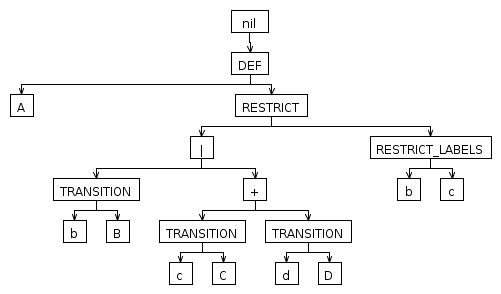
\includegraphics[width=3.5in]{ast_example}
% where an .eps filename suffix will be assumed under latex, 
% and a .pdf suffix will be assumed for pdflatex; or what has been declared
% via \DeclareGraphicsExtensions.
\caption{AST Example}
\label{fig:ast_example}
\end{figure}

No tralalal \ref{eq:ccs_example}..
